\documentclass{standalone}
\usepackage{tikz}
\usetikzlibrary{patterns, positioning}
\usepackage[sfdefault]{ClearSans} %% option 'sfdefault' activates Clear Sans as the default text font
\usepackage[T1]{fontenc}

\begin{document}
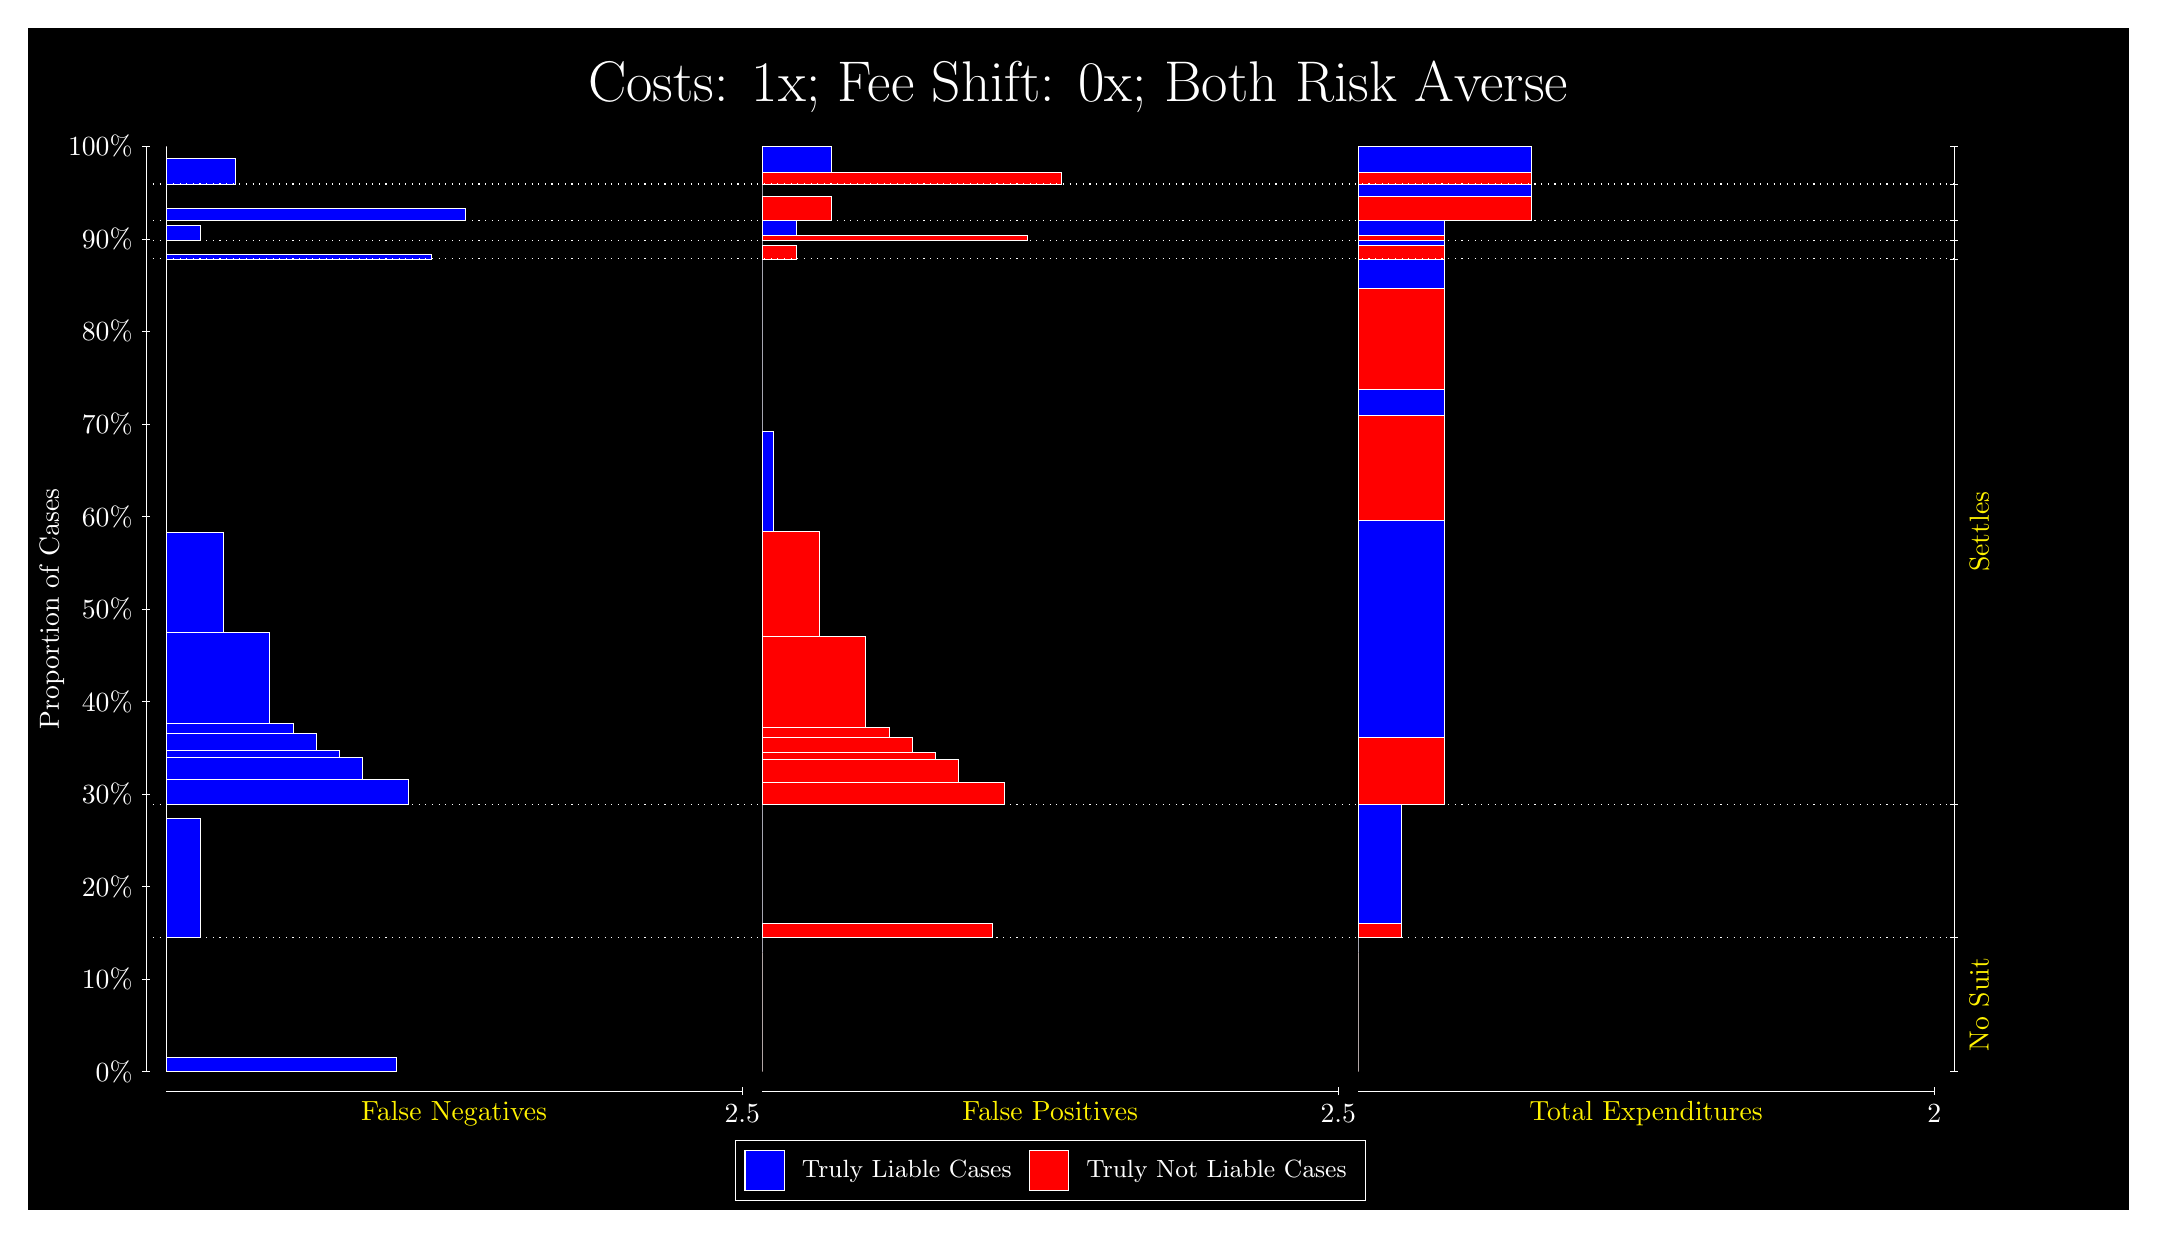
\begin{tikzpicture}
\draw[fill=black] (0,0) rectangle (26.667,15);
\draw[text=white] (0,13.5) rectangle (26.667,15) node[midway] {\huge Costs: 1x; Fee Shift: 0x; Both Risk Averse};
\draw[white, very thin] (1.5,1.75) -- (1.5,13.5);
\node[rotate=90, text=white, anchor=center] at (0.3, 7.625) {Proportion of Cases};
\draw[white, very thin] (1.45,1.75) -- (1.55,1.75);
\node[text=white, anchor=east] at (1.45, 1.75) {0\%};
\draw[white, very thin] (1.45,2.925) -- (1.55,2.925);
\node[text=white, anchor=east] at (1.45, 2.925) {10\%};
\draw[white, very thin] (1.45,4.1) -- (1.55,4.1);
\node[text=white, anchor=east] at (1.45, 4.1) {20\%};
\draw[white, very thin] (1.45,5.275) -- (1.55,5.275);
\node[text=white, anchor=east] at (1.45, 5.275) {30\%};
\draw[white, very thin] (1.45,6.45) -- (1.55,6.45);
\node[text=white, anchor=east] at (1.45, 6.45) {40\%};
\draw[white, very thin] (1.45,7.625) -- (1.55,7.625);
\node[text=white, anchor=east] at (1.45, 7.625) {50\%};
\draw[white, very thin] (1.45,8.8) -- (1.55,8.8);
\node[text=white, anchor=east] at (1.45, 8.8) {60\%};
\draw[white, very thin] (1.45,9.975) -- (1.55,9.975);
\node[text=white, anchor=east] at (1.45, 9.975) {70\%};
\draw[white, very thin] (1.45,11.15) -- (1.55,11.15);
\node[text=white, anchor=east] at (1.45, 11.15) {80\%};
\draw[white, very thin] (1.45,12.325) -- (1.55,12.325);
\node[text=white, anchor=east] at (1.45, 12.325) {90\%};
\draw[white, very thin] (1.45,13.5) -- (1.55,13.5);
\node[text=white, anchor=east] at (1.45, 13.5) {100\%};

\draw[white, very thin] (24.457,1.75) -- (24.457,13.5);
\draw[white, very thin] (24.407,1.75) -- (24.507,1.75);
\node[anchor=west] at (24.407, 1.75) {};
\draw[white, very thin] (24.407,3.4516) -- (24.507,3.4516);
\node[anchor=west] at (24.407, 3.4516) {};
\draw[white, very thin] (24.407,5.1407) -- (24.507,5.1407);
\node[anchor=west] at (24.407, 5.1407) {};
\draw[white, very thin] (24.407,12.07) -- (24.507,12.07);
\node[anchor=west] at (24.407, 12.07) {};
\draw[white, very thin] (24.407,12.308) -- (24.507,12.308);
\node[anchor=west] at (24.407, 12.308) {};
\draw[white, very thin] (24.407,12.559) -- (24.507,12.559);
\node[anchor=west] at (24.407, 12.559) {};
\draw[white, very thin] (24.407,13.021) -- (24.507,13.021);
\node[anchor=west] at (24.407, 13.021) {};
\draw[white, very thin] (24.407,13.5) -- (24.507,13.5);
\node[anchor=west] at (24.407, 13.5) {};

\draw[white, very thin, fill=blue] (1.75,1.75) rectangle (4.6775,1.9368);
\draw[white, very thin, fill=red] (1.75,1.9368) rectangle (1.75,3.4516);
\draw[white, very thin, fill=blue] (1.75,3.4516) rectangle (2.1891,4.9601);
\draw[white, very thin, fill=red] (1.75,4.9601) rectangle (1.75,5.1407);
\draw[white, very thin, fill=blue] (1.75,5.1407) rectangle (4.8239,5.4637);
\draw[white, very thin, fill=blue] (1.75,5.4637) rectangle (4.2384,5.7464);
\draw[white, very thin, fill=blue] (1.75,5.7464) rectangle (3.9457,5.8353);
\draw[white, very thin, fill=blue] (1.75,5.8353) rectangle (3.6529,6.0403);
\draw[white, very thin, fill=blue] (1.75,6.0403) rectangle (3.3602,6.1725);
\draw[white, very thin, fill=blue] (1.75,6.1725) rectangle (3.0674,7.3279);
\draw[white, very thin, fill=blue] (1.75,7.3279) rectangle (2.4819,8.5944);
\draw[white, very thin, fill=red] (1.75,8.5944) rectangle (1.75,12.07);
\draw[white, very thin, fill=blue] (1.75,12.07) rectangle (5.1167,12.133);
\draw[white, very thin, fill=red] (1.75,12.133) rectangle (1.75,12.308);
\draw[white, very thin, fill=blue] (1.75,12.308) rectangle (2.1891,12.492);
\draw[white, very thin, fill=red] (1.75,12.492) rectangle (1.75,12.559);
\draw[white, very thin, fill=blue] (1.75,12.559) rectangle (5.5558,12.711);
\draw[white, very thin, fill=red] (1.75,12.711) rectangle (1.75,13.021);
\draw[white, very thin, fill=blue] (1.75,13.021) rectangle (2.6283,13.348);
\draw[white, very thin, fill=red] (1.75,13.348) rectangle (1.75,13.5);
\draw[white, very thin, fill=red] (9.3189,1.75) rectangle (9.3189,3.2648);
\draw[white, very thin, fill=blue] (9.3189,3.2648) rectangle (9.3189,3.4516);
\draw[white, very thin, fill=red] (9.3189,3.4516) rectangle (12.246,3.6322);
\draw[white, very thin, fill=blue] (9.3189,3.6322) rectangle (9.3189,5.1407);
\draw[white, very thin, fill=red] (9.3189,5.1407) rectangle (12.393,5.4267);
\draw[white, very thin, fill=red] (9.3189,5.4267) rectangle (11.807,5.7094);
\draw[white, very thin, fill=red] (9.3189,5.7094) rectangle (11.515,5.7983);
\draw[white, very thin, fill=red] (9.3189,5.7983) rectangle (11.222,5.9935);
\draw[white, very thin, fill=red] (9.3189,5.9935) rectangle (10.929,6.1257);
\draw[white, very thin, fill=red] (9.3189,6.1257) rectangle (10.636,7.2811);
\draw[white, very thin, fill=red] (9.3189,7.2811) rectangle (10.051,8.6167);
\draw[white, very thin, fill=blue] (9.3189,8.6167) rectangle (9.4652,9.8832);
\draw[white, very thin, fill=blue] (9.3189,9.8832) rectangle (9.3189,12.07);
\draw[white, very thin, fill=red] (9.3189,12.07) rectangle (9.758,12.245);
\draw[white, very thin, fill=blue] (9.3189,12.245) rectangle (9.3189,12.308);
\draw[white, very thin, fill=red] (9.3189,12.308) rectangle (12.686,12.374);
\draw[white, very thin, fill=blue] (9.3189,12.374) rectangle (9.758,12.559);
\draw[white, very thin, fill=red] (9.3189,12.559) rectangle (10.197,12.868);
\draw[white, very thin, fill=blue] (9.3189,12.868) rectangle (9.3189,13.021);
\draw[white, very thin, fill=red] (9.3189,13.021) rectangle (13.125,13.173);
\draw[white, very thin, fill=blue] (9.3189,13.173) rectangle (10.197,13.5);
\draw[white, very thin, fill=red] (16.888,1.75) rectangle (16.888,3.2648);
\draw[white, very thin, fill=blue] (16.888,3.2648) rectangle (16.888,3.4516);
\draw[white, very thin, fill=red] (16.888,3.4516) rectangle (17.437,3.6322);
\draw[white, very thin, fill=blue] (16.888,3.6322) rectangle (17.437,5.1407);
\draw[white, very thin, fill=red] (16.888,5.1407) rectangle (17.986,5.9935);
\draw[white, very thin, fill=blue] (16.888,5.9935) rectangle (17.986,8.7526);
\draw[white, very thin, fill=red] (16.888,8.7526) rectangle (17.986,10.088);
\draw[white, very thin, fill=blue] (16.888,10.088) rectangle (17.986,10.411);
\draw[white, very thin, fill=red] (16.888,10.411) rectangle (17.986,11.699);
\draw[white, very thin, fill=blue] (16.888,11.699) rectangle (17.986,12.07);
\draw[white, very thin, fill=red] (16.888,12.07) rectangle (17.986,12.245);
\draw[white, very thin, fill=blue] (16.888,12.245) rectangle (17.986,12.308);
\draw[white, very thin, fill=red] (16.888,12.308) rectangle (17.986,12.374);
\draw[white, very thin, fill=blue] (16.888,12.374) rectangle (17.986,12.559);
\draw[white, very thin, fill=red] (16.888,12.559) rectangle (19.083,12.868);
\draw[white, very thin, fill=blue] (16.888,12.868) rectangle (19.083,13.021);
\draw[white, very thin, fill=red] (16.888,13.021) rectangle (19.083,13.173);
\draw[white, very thin, fill=blue] (16.888,13.173) rectangle (19.083,13.5);
\draw[white, dotted] (1.5,3.4516) -- (24.457,3.4516);
\draw[white, dotted] (1.5,5.1407) -- (24.457,5.1407);
\draw[white, dotted] (1.5,12.07) -- (24.457,12.07);
\draw[white, dotted] (1.5,12.308) -- (24.457,12.308);
\draw[white, dotted] (1.5,12.559) -- (24.457,12.559);
\draw[white, dotted] (1.5,13.021) -- (24.457,13.021);
\draw[white, very thin] (1.75,1.5) -- (9.0689,1.5);
\node[text=yellow, anchor=north] at (5.4094, 1.5) {False Negatives};
\draw[white, very thin] (9.0689,1.45) -- (9.0689,1.55);
\node[text=white, anchor=north] at (9.0689, 1.45) {2.5};

\draw[white, very thin] (9.3189,1.5) -- (16.638,1.5);
\node[text=yellow, anchor=north] at (12.978, 1.5) {False Positives};
\draw[white, very thin] (16.638,1.45) -- (16.638,1.55);
\node[text=white, anchor=north] at (16.638, 1.45) {2.5};

\draw[white, very thin] (16.888,1.5) -- (24.207,1.5);
\node[text=yellow, anchor=north] at (20.547, 1.5) {Total Expenditures};
\draw[white, very thin] (24.207,1.45) -- (24.207,1.55);
\node[text=white, anchor=north] at (24.207, 1.45) {2};

\node[text=yellow, centered, rotate=90] at (24.777, 2.6008) {No Suit};

\node[text=yellow, centered, rotate=90] at (24.777, 8.6055) {Settles};





\draw (12.978300999999998,1.5) node[draw=none] (baseCoordinate) {};
\begin{scope}[align=center]
        \matrix[scale=0.5, draw=white, below=0.5cm of baseCoordinate, nodes={draw}, column sep=0.1cm]{
            \node[rectangle, draw, minimum width=0.5cm, minimum height=0.5cm, fill=blue] {}; &
            \node[draw=none, font=\small, text=white] (B) {Truly Liable Cases}; &
            \node[rectangle, draw, minimum width=0.5cm, minimum height=0.5cm, fill=red] {}; &
            \node[draw=none, font=\small, text=white] (B) {Truly Not Liable Cases}; \\
            };
\end{scope}

\end{tikzpicture}
\end{document}